\subsection{Drifting Clocks and Clock Synchronization}
\label{subsec:drifting-clocks-and-synchronization}

We assume the existence of ``nominal time'' (cf.~\cite{EC:BGKRZ21,TCC:GarKiaShe22}, also known as ``real time'' or ``Newtonian time'' \cite{JCSS:DHS86}), which is not directly observable by protocol participants.
%
Following the traditional assumption in distributed computing that each party is equipped with a physical clock, whose output is a real-valued function of nominal time, in this paper we consider the \textbf{drifting clock} model.
%
Specifically, honest parties possess physical clocks with a bounded rate of drift from nominal time (\cref{fig:drifting-clocks}) --- i.e., an honest physical clock stays within a \emph{linear envelope} of nominal time.\footnote{A function $f: \mathbb{R} \rightarrow \mathbb{R}$ is within a $(U, L)$-linear envelope if and only if it holds that $L \cdot x - c \leq f(x)\leq U \cdot x + c$, where $c$ is a constant and $x \in \mathbb{R}^+$.}
%
We use \clockDrift to denote the bound on the rate of honest physical clocks.
% 
Formally, for any nominal time $u > v$ and an honest physical clock $D$, it holds that
%
\[ (1 + \clockDrift)^{-1} (u - v) \le D(u) - D(v) \le (1 + \clockDrift) (u - v). \]

\begin{figure}[ht]
    \centering
    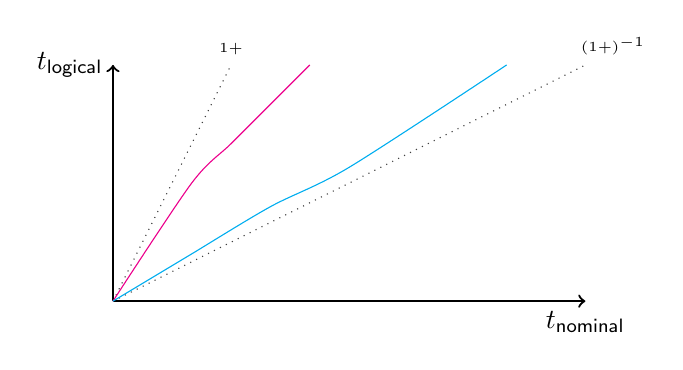
\begin{tikzpicture}
        \draw[->, thick] (0, 0) -- (6, 0) node[below] {$t_{\mathsf{nominal}}$};
        \draw[->, thick] (0, 0) -- (0, 3) node[left] {$t_{\mathsf{logical}}$};

        \draw[dotted, color = darkgray] (0, 0)--(6, 3) node[above, color = black, xshift=1em] {\tiny $(1 + \clockDrift)^{-1}$};
        \draw[dotted, color = darkgray] (0, 0)--(1.5, 3) node[above, color = black] {\tiny $1 + \clockDrift$};

        \draw[opacity=0]  (0,0) -- (1,1) -- (1.5, 2) -- (2, 2.5)  -- (3, 3);

        \draw [magenta] plot [smooth] coordinates { (0,0) (1,1.5) (1.5, 2) (2, 2.5) (2.5, 3)};

        \draw [cyan] plot [smooth] coordinates { (0, 0) (0.5, 0.3) (1, 0.6) (2, 1.2) (3, 1.7) (5, 3)};
    \end{tikzpicture}

    \caption{An illustration of drifting clocks within a $(0.5, 2)$-linear envelope (i.e., $\clockDrift = 1$). Without clock synchronization, two clocks (illustrated in magenta and cyan, respectively) deviate from each other unboundedly.}
    \label{fig:drifting-clocks}
\end{figure}


Note that time in the drifting clock model are real values, while our protocol execution model divides time into discrete integer-numbered steps.
%
In order to ``insert'' real-valued time into this structure, we model drifting local clocks as \funcDriftingClock, derived from the global clock functionality in~\cite{TCC:KMTZ13}.
%
In \funcDriftingClock, nominal time is defined by the number of times that the clock functionality moves forward the time-step variable $\tau$ (which is an internal variable and is unknown to the parties).
%
Instead of directly receiving the time from \funcDriftingClock, parties receive ``ticks'' from \funcDriftingClock which indicates that they should advance their local round number.
%
\funcDriftingClock advances the nominal time when all (honest) participants claim they have finished their computation in the current round.
%
Additionally, \funcDriftingClock allows the adversary to ``push'' or ``stall'' honest clocks, as long as these operations do not violate the \clockDrift-bounded linear envelope assumption.
%
We present \funcDriftingClock in~\cref{functionality:drifting-clock}.

\begin{remark}
    As opposed to the classical distributed computing setting (cf.~\cite{JACM:DwoLynSto88}) where rounds/time steps are defined as intervals of equal length in the view of an external real-time clock, in our model \funcDriftingClock does not guarantee that rounds/time steps are of equal duration.
    %
    In fact, the notions of `time' and `duration' are not defined in the UC setting.
    %
    Yet, our model shows the same effect in restricting local clock counters staying in a bounded linear envelope with respect to the nominal clock counter; moreover, the same amount of computation is carried out per local time counter increment --- which means that in the same window of nominal time, a faster CPU will solve more PoWs than a slower one.
\end{remark}

\begin{cccFunctionality}
    {\funcDriftingClock}
    {drifting-clock}
    {The drifting global clock.}

    This functionality maintains state variables as follows.

    \addtocounter{table}{-1}
    \begin{tabularx}{.9\textwidth}{c X}
        \toprule[.3mm]
        \textbf{State Variable}
         & \textbf{Description}
        \\ \midrule[.3mm]
        $\clockDrift \gets 0$
         & The bound on clock drifts.
        \\ \midrule
        $\partyset \gets \emptyset$
         & The set of registered parties $\party = (\pid, \sid)$.
        \\ \midrule
        $F \gets \emptyset$
         & The set of registered functionalities (together with their session identifier).
        \\ \midrule
        $\tau_\sid \gets 0$
         & The nominal-time variable for session \sid.
        \\ \midrule
        $d_\party \gets 0$
         & The clock-update variable for $\party = (\pid, \sid) \in \partyset$.  $d_\party$ is set to $1$ after \party finishes a round.
        \\ \midrule
        $b_\party \gets 1$
         & The tick-budget variable for $\party = (\pid, \sid) \in \partyset$.
        \\ \midrule
        $d(\F, \sid) \gets 0$
         & The clock-update variable for $(\F, \sid) \in F$.
        \\ \bottomrule[.3mm]
    \end{tabularx}

    \paragraph{Setting the drift:}
    %
    \begin{cccItemize}[nosep]
        \item Upon  receiving $(\textsc{set-drift}, \sid, r)$ from the adversary \adv, \textbf{if} \textsc{set-drift} has never been received then set $\clockDrift = r$. Return $(\textsc{set-drift}, \sid, \ok)$ to \adv.
    \end{cccItemize}

    \paragraph{Clock capabilities:}
    %
    \begin{cccItemize}[nosep]
        \item Upon receiving $(\textsc{clock-update}, \sid_C)$ from some party $\party \in \partyset$ set $d_\party \gets 1$ and $b_\party \gets b_\party - 1$; execute \textit{Time-Update} and forward $(\textsc{clock-update}, \sid_C , \party)$ to \adv.

        \item Upon receiving $(\textsc{clock-update}, \sid_C)$ from some functionality \F in a session \sid such that $(\F, \sid) \in F$ set $d(\F, \sid) \gets 1$, execute \emph{Time-Update} and return $(\textsc{clock-update},\allowbreak \sid_C, \F)$ to this instance of \F.

        \item Upon receiving $(\textsc{clock-forward}, \sid_C , \party)$ from \adv where $\party \in \partyset$, if $d_\party = 0$ or it is about to violate the \clockDrift-bounded linear envelope on \party, ignore the message.
        %
        Otherwise, update $d_\party = 0$ and $b_\party \gets b_\party + 1$; return $(\textsc{clock-forward-ok}, \sid_C , \party)$ to \adv.

        \item Upon receiving $(\textsc{clock-backward}, \sid_C , \party)$ from \adv where $\party \in \partyset$, if $d_\party = 0$ or it is about to violate the \clockDrift-bounded linear envelope on \party, ignore the message.
        %
        Otherwise, update $b_\party \gets b_\party - 1$; return $(\textsc{clock-backward-ok}, \sid_C , \party)$ to \adv.

        \item Upon receiving $(\textsc{clock-tick}, \sid_C)$ from any participant \party --- including the environment on behalf of a party --- or the adversary on behalf of a corrupted party \party (resp. from any ideal---shared or local---functionality \F), execute procedure \textit{Time-Update}, return $(\textsc{clock-tick}, \sid_C, d_{\party})$ (resp. $(\textsc{clock-tick}, \sid_C, d_{(\F, \sid)})$) to the requestor (where \sid is the session id of the calling instance).

        \item Upon receiving $(\textsc{clock-read}, \sid_C)$ from the adversary or the wapper functionalities, return $(\textsc{clock-read},\sid_C, \tau_{\sid})$ to the requestor (where \sid is the session id of the calling instance).
    \end{cccItemize}

    \medskip\emph{Procedure Time-Update:}
    %
    For each session \sid do: If (i) $d_{(\func, \sid)} = 1$ for all $\func \in F$, and (ii) $d_\party = 1$ and $b_\party \le 0$ for all honest parties $\party = (\cdot, \sid) \in \partyset$, then update $\tau_\sid \gets \tau_\sid + 1$, $d_{(\func,\sid)} \gets 0$ and $b_\party \gets b_\party + 1$ for all parties $\party = (\cdot, \sid) \in \partyset$.
    %
    Additionally, for all parties $\party = (\cdot, \sid) \in \partyset$ with $b_\party > 0$, update $d_\party \gets 0$.
\end{cccFunctionality}


We adapt the traditional definition of the clock synchronization problem (cf.~\cite{JCSS:DHS86,JACM:SriTou87}) to our permissionless setting.
%
In~\cref{def:clock-properties}, we consider two properties, \emph{bounded skew} and \emph{accuracy}, that establish upper bounds \maxSkew and $\varGamma$ on honest clock skew and their deviation from the nominal time, respectively.

\begin{definition}
    [Clock Synchronization]
    \label{def:clock-properties}
    There exist constants $\maxSkew \in \mathbb{N}$, $\varGamma \in \mathbb{R}^+$ such that honest parties' logical clocks satisfy the following two properties:
    %
    \begin{cccItemize}[nosep]
        \item \emph{\bf Bounded skew (with parameter $\maxSkew \in \mathbb{N}$).}
        %
        Let $\round_1, \round_2$ be the reported logical clocks of two
        honest parties at any nominal time $r$.
        %
        Then $|\round_ 1 - \round_2| \le \maxSkew$.

        \item \emph{\bf Accuracy (with parameter $\varGamma \in \mathbb{R}^+$).}
        %
        Each honest party's logical clock stays in a $(U, L)$-linear envelope with respect to the nominal time $r$, where $U = 1 + \varGamma$ and $L = 1 / (1 + \varGamma)$.
    \end{cccItemize}
\end{definition}
